\chapter{Preliminares} \label{preliminares}
En el campo del machine learning los algoritmos más usados son las redes neuronales. Con este tipo de algoritmos los ordenadores son capaces de realizar predicciones, encontrar patrones y replicar acciones que un ser humano puede hacer, como por ejemplo: el reconocimiento y la clasificación de objetos. Para que las redes neuronales puedan hacer estas tareas es necesario realizar un entrenamiento con grandes conjuntos de datos. En el proceso de entrenamiento a la red neuronal (en el caso del aprendizaje supervisado) se le muestra ejemplos de los problemas que tiene que resolver junto a su solución y en función de si ha conseguido resolver o no el problema, la red se actualizará. Pero, ¿qué es una red neuronal?.

\section{Redes neuronales}
Una red neuronal \cite{RefWorks:RefID:22-jain1996artificial} es un sistema de cómputo que consiste en un grafo dirigido ponderado en el que las neuronas artificiales son los nodos del grafo y los pesos de la red son las  aristas ponderadas que conectan la salida de las neuronas con las entradas. Estas neuronas están formadas por dendritas (las conexiones de entrada) y por los axones (las conexiones de salida). Dentro de cada una de estas neuronas se realiza una suma ponderada con los pesos de las dendritas, y tras aplicarle una función de activación, se transmite el resultado a las neuronas de la siguiente capa por los axones. 

\begin{figure}
    \centering
    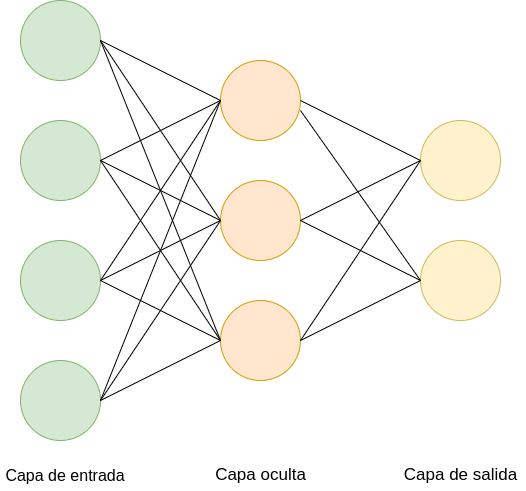
\includegraphics[width=0.5\textwidth]{imagenes/fdnn.drawio.png} 
    \caption{Red neuronal}
\end{figure}

El objetivo de entrenar una red neuronal es conseguir ajustar los pesos de la red para conseguir resolver problemas, ya sean de regresión, clasificación o una combinación de ambos. Los métodos que se usan para enseñar a la redes neuronales se conocen como algoritmos de entrenamiento. Un buen algoritmo de entrenamiento tiene que ser capaz de poder mejorar el desempeño de la red neuronal haciendo uso de los datos de entrenamiento del problema.

Actualmente el algoritmo más usado es el backpropagation \cite{RefWorks:RefID:6-rumelhart1986learning} debido a su capacidad de encontrar buenos resultados y a su eficiencia. Desde que se inventó este algoritmo ha sido el más estudiado creándose numerosas variantes cuyo objetivo era el de mejorar los puntos débiles de este algoritmo, como son su inviabilidad biológica, el problema del transporte de pesos \cite{RefWorks:RefID:10-grossberg1987competitive} y el desvanecimiento de gradientes.

Haciendo una revisión en la literatura actual nos podemos encontrar con algunos de los algoritmos más populares como son el grupo de los métodos quasi-newton, el método del gradiente conjugado\cite{RefWorks:RefID:13-johansson1991backpropagation} y el algoritmo de Levenberg-Marquardt\cite{yu2011levenberg}.

\section{Métodos Quasi-Newton}

Los métodos quasi-newton son aproximaciones al método de Newton. La motivación de estos algoritmos es conseguir aplicar de manera práctica el método de Newton a problemas de machine learning actuales. El gran problema que tiene el método de Newton es su alto coste computacional, ya que hace uso de la derivada segunda para la optimización de funciones, es decir, necesita realizar el cálculo de la matriz Hessiana. En problemas con un número de variables grande es imposible aplicar este algoritmo. Por este motivo surgen los métodos quasi-newton, los cuales abordan el problema del cálculo de la matriz Hessiana mediante aproximaciones. Dentro del conjunto de estos algoritmos uno de los más conocidos es el L-BFGS \cite{RefWorks:RefID:12-rafati2018improving} (Limited-Broyden–Fletcher–Goldfarb–Shanno), el cual aproxima la matriz Hessiana iterativamente creando un proceso mucho más eficiente. 

\section{Gradiente Conjugado}

El gradiente conjugado es un algoritmo que se encuentra entre el gradiente descendente y el método de newton. La motivación de este algoritmo es solucionar la convergencia lenta del gradiente descendente y evitar los requerimientos del cálculo de la matriz Hessiana como invertir la matriz, evaluarla y almacenarla. 

\section{Método Levenberg-Marquardt}

Finalmente, el método del Levenberg-Marquardt esta diseñado para trabajar con la función de pérdida. No necesita calcular la matriz Hessiana, sino que calcula el vector gradiente y la matriz Jacobiana.

Además de los métodos ya mencionados, existen alternativas que se centran en mejorar el propio backpropagation como puede ser el algoritmo Adadelta \cite{https://doi.org/10.48550/arxiv.1212.5701}, el cual modifica el comportamiento del learning rate para mejorar la convergencia y los resultados que obtiene. 

Hasta ahora hemos analizando alternativas que no son muy viables computacionalmente para los problemas de hoy en día o algoritmos que no son alternativas como tal, si no más bien mejoras del propio backpropagation. A pesar de que estos ejemplos son los más ampliamente usados existen alternativas que no son tan usadas pero si suponen una alternativa real para el backpropagation. Estos son los algoritmos en los que se van a centrar el proyecto, pues el objetivo es estudiar como distintos algoritmos de entrenamiento se comportan bajo las condiciones de la cuantización. Los algoritmos seleccionados para este estudio son:  el HSIC Bottleneck \cite{ma2020hsic}, el feedback alignment \cite{RefWorks:RefID:9-lillicrap2016random} y synthetic gradients \cite{jaderberg2017decoupled}. Se tratan de algoritmos recientes (2016-2020) los cuales han conseguido buenos resultados. La descripción y análisis se realizará en los siguientes apartados.  

Vista la actualidad del entrenamiento de redes neuronales nos toca centrarnos en los otros dos aspectos que involucran este proyecto: la cuantificación de redes neuronales y la aplicación de redes neuronales en la computación neuromórfica.

La cuantificación de redes neuronales es un campo de estudio que se encuentra en auge debido a cuestiones como el tamaño que ocupan los modelos y las velocidades de inferencia. Hoy en día los modelos más punteros consisten en arquitecturas de varios gigas de tamaño, por lo que solo pueden ser ejecutadas en equipos que cuenten con la capacidad de almacenamiento y de cómputo necesarias para realizar las inferencias. Estas restricciones provoca que dispositivos móviles no puedan usar este tipo de redes de forma nativa. 

Con el objetivo de reducir los tamaños y aumentar las velocidades de inferencia se crean los métodos de cuantificación. Estos técnicas consisten en reducir la precisión numérica de la red, cuantificando los pesos y en ocasiones las operaciones dentro de la red. El proceso de cuantificar consiste en transformar los números de alta precisión en enteros de 1-8 bits, para ello existen varios métodos que se pueden dividir en procesos determinísticos y probabilísticos. Los procesos determinísticos mapean los números de alta precisión en el espacio de los números enteros de baja precisión, existiendo una relación de 1 a 1, un ejemplo es el método de redondeo que se usa en el BinaryConnect \cite{10.5555/2969442.2969588}, donde se realiza una cuantificación binaria en función del signo. Por otro lado, los procesos probabilísticos usan distribuciones de probabilidad para realizar las cuantificaciones por lo que un número no siempre se cuantificará de la misma manera, ejemplo de este tipo de cuantificaciones se puede encontrar en \cite{10.5555/2969442.2969588} en el que la cuantificación estocástica se realiza en base a una distribución de probabilidad. La intuición es que si el valor es positivo existe una alta probabilidad de que su valor final sea 1, pero también cabe la posibilidad de que se cuantifique como -1. 

Otro elemento importante de la cuantificación de redes neuronales es el momento en el que se aplican dichas cuantificaciones, pudiendo realizarse la cuantificación durante el entrenamiento o durante la inferencia. Durante el entrenamiento la cuantificación se aplica durante el feedforward pass y durante el backward pass mientras se realiza el entrenamiento. Implementaciones de este tipo de cuantificaciones nos lo podemos encontrar en estudios como el ya mencionado BinaryConnect, donde se entrena una red binaria y en XNOR-Net \cite{Rastegari2016XNORNetIC} que aplica redes binarias a problemas más grandes como ImageNet. Por su parte la redes que usan cuantificación después del entrenamiento no aplican ninguna cuantificación a su entrenamiento, la red una vez entrenada es cuantificada para reducir su tamaño y acelerar la inferencia. Ejemplos de este tipo de cuantificaciones son: DeepCompression \cite{DBLP:journals/corr/HanMD15}, reduce el tamaño de la red podando conexiones irrelevantes y los pesos restantes los cuantifica a valores discretos; Entropy-constrained scalar quantization \cite{DBLP:conf/iclr/ChoiEL17}, tiene en cuenta la información de la segunda derivada de la función de pérdida para medir la importancia de los distintos pesos, y la cuantificación se realiza a través de técnicas de clustering; e Incremental network quantization \cite{DBLP:journals/corr/ZhouYGXC17}, cuyo proceso de cuantificación se divide en tres partes: partición de pesos, cuantificación por grupo y reentreno. \cite{https://doi.org/10.48550/arxiv.1808.04752}

El último campo que queda por revisar es el de la computación neuromórfica, centrando la atención al estudio de la aplicación de redes neuronales a este tipo de circuitos. 

En la actualidad la computación neuromórfica se encuentra en auge debido a los problemas anteriormente mencionados: ralentizacion de la ley de Moore, el memory wall problem y la contaminación producida por los procesos de entrenamiento de redes neuronales; y a sus  grandes ventajas: alto nivel de paralelismo, escalabilidad inherente, computación dirigida por eventos y estocasticidad. Sin embargo, la computación neuromórfica se encuentra en una temprana edad y las numerosas investigaciones que se han realizado están lejos de la fase de producción. Dentro de estos estudios los frameworks más destacados son: TrueNorth \cite{7229264}, SpiNNaker \cite{6750072} y Loihi \cite{8259423}. En el estudio de TrueNorth se han centrado en la aplicación de spiking neural networks \cite{doi:10.1142/S0129065709002002}, esta red es entrenada off-chip, es decir, no se entrenaba en el propio circuito y después se transformaba para ejecutarse en el circuito neuromórfico. SpiNNaker también aplica spiking neurons teniendo como ventaja principal una mayor flexibilidad en la elección de la topología de la red y el tipo de neurona a usar. Loihi al igual que los anteriores aplica las spiking neurons pero tiene como novedad el entrenamiento on-chip. Las otras redes que se aplican en los circuitos neuromórficos son las fully connected y las convolutional neural networks, investigado como afecta la cuantificación a las redes una vez ya entrenadas. En este estudio \cite{10481/72221} se ve como afecta la reducción de la precisión numérica de los pesos al rendimiento final de la red. Por otro lado, existen investigaciones que además estudian como afecta la cuantificación si se introduce en el entrenamiento \cite{8705375}. Cabe destacar que para las redes fully connected solo se usan redes binarias mientras que la cuantificación de varios niveles solo se estudia en las redes convolucionales. \cite{DBLP:journals/corr/SchumanPPBDRP17}

\section{Algoritmos preliminares}

Este apartado esta destinado a explicar los métodos, algoritmos o herramientas que se van a utilizar en los algoritmos a estudiar con el objetivo de no tener que repetir su significado o funcionamiento.

\subsection{Propagación hacia delante}

La propagación forward o hacia delante es el proceso que se realiza para calcular la hipótesis de la red neuronal. Consiste en ir pasando la información de capa a capa, empezando por la inicial y llegando hasta la de salida. El proceso que se lleva a cabo es multiplicar la entrada por la matriz de pesos de la primera capa, a este resultado se le aplica la función de activación que se esté usando en la red. Este proceso se repite hasta llegar a la capa final, en la que la función de activación dependiendo del problema puede ser la identidad, softmax, entropía cruzada, etc.

\begin{algorithm}[H]
   \caption{Propagación hacia delante}
   \KwData{x: dato de entrada, $w = \{W^{1}, ..., W^{L}\}$: matrices de pesos, \\$\theta$: función de activación}
   \KwResult{h(x): hipótesis }
   
   $x^{(0)} \gets x$ \\
   \For{l = 1 to L }{
        $s^{(l)} \gets (W^{(l)})^{T}x^{(l-1)}$ \\
        $x^{(l)} \gets $ 
        $
        \begin{bmatrix}
        1 \\
        \theta(s^{(l)})
        \end{bmatrix}
        $
   } 
   $h(x) = x^{(L)}$
   \label{tab:Feedforward}
\end{algorithm}

\subsection{Gradiente descendente}

El gradiente descendente es una técnica básica de optimización de funciones en los algoritmos de machine learning. Consiste en calcular el mínimo de una función de forma iterativa haciendo uso de la derivada de la función a estudiar. 

La ejecución del algoritmo se inicia desde un punto aleatorio de la función. Para dirigirse hacia el mínimo más cercano el algoritmo calcula la derivada de la función en dicho punto y se desplaza en sentido contrario a esta. 

\begin{algorithm}[H]
   \caption{Gradiente descendente}
   \KwData{$w_{0}$: punto de partida; $\theta$: función a optimizar; $max\_iter$: numero máximo de iteraciones; $\eta$ learning rate}
   \KwResult{un mínimo de la función}
   $w \gets x_{0}$\\
   \For{i = 1 hasta $max\_iter$ }{
        $w = w - \eta f'(w)$
   } 
\end{algorithm}
\section{Algoritmos}

A continuación presento los algoritmos de entrenamiento que se van a estudiar para este proyecto.

\subsection{Backpropagation} \label{tab:Backprop}

El algoritmo Backpropagation, abreviatura de ``backward propagation error", es un algoritmo de aprendizaje supervisado para redes neuronales que hace uso del gradiente descendente. Se trata de una generalización de la regla delta del perceptron para las redes neuronales multicapa. Su funcionamiento se basa en calcular el gradiente de la función de error con respecto a los pesos de la red. Para calcular los gradientes de cada capa primero se calculan los vectores de sensibilidad los cuales cuantifican cuanto cambia el error con respecto a $s^{(l)}$ siendo $s^{(l)} = (W^{(L)})x^{(l-1)}$ el resultado de multiplicar los pesos de la capa $l$, $W^{(L)}$, con el resultado de la capa $l-1$, $x^{(l-1)}$. Calculadas las sensibilidades el siguiente paso es calcular los gradientes, para ello se multiplicara cada vector de sensibilidad, $\delta^{(l)}$, por los resultados de cada capa, $x^{(l)}$. Finalmente para actualizar la red se usará la regla del gradiente descendente.

\begin{algorithm}[H]
   \caption{Backpropagation para calcular la sensibilidad}
   \KwData{Un punto de la muestra $(x,y)$; las matrices de pesos, $w = \{W^{1},...,W^{L}\}$; la función de activación $\theta$}
   \KwResult{La sensibilidad  $\delta^{(l)}$ para $l = \{L,...,1\}$}
   Ejecutamos el proceso Feedforward \ref{tab:Feedforward} para obtener:\\
   $s^{(l)}$ para $l = \{L,...,1\}$ \\
   $x^{(l)}$ para $l = \{L,...,1\}$ \\  
   $\delta^{(L)} \gets 2(x^{(L)-y})\theta'(s^{(L)})$ \\
   \For{$l = L - 1$ hasta $1$}{
        $\delta^{(l)} = \theta'(s^{(l)}) \otimes [W^{(l+1)}\delta^{(l+1)}]$
   }
   
   \label{tab:Backprop_alg}
\end{algorithm}

\begin{algorithm}[H]
   \caption{Proceso del calculo de gradientes $g = \nabla E_{in}(w)$ y la función de error $E_{in}(w)$}
   \KwData{$w = \{W^{1},...,W^{L}\}$; $D = (x_{1},y_{1}) ... (x_{N},y_{N})$}
   \KwResult{el error $E_{in}(w)$ y los gradientes $g = \{G^{1},...,G^{L}\}$}
   Inicialización: $E_{in} = 0$ y $G^{(l)} = 0 $ para $l = 1,...,L$ \\
   \For{por cada punto en la muestra $(x_{n}, y_{n}), n = 1,...,N$}{
        Calculamos $x^{(l)}$ para $l = 1,...,L$ [forward propagation] \ref{tab:Feedforward} \\
        Calculamos $\delta^{(l)}$ para $l = 1,...,L$ [backpropagation] \ref{tab:Backprop_alg} \\
        \For{$l = 1,...,L$}{
            $G^{(l)}(x_{n}) = [x^{(l-1)}(\delta^{(l)})^{T}]$ \\
            $G^{(l)} \gets G^{(l)} + \frac{1}{N}G^{(l)}(x_{n}) $
        }
        
   }
\end{algorithm}

La actualización de los pesos se hará con el uso del gradiente descendente el cual dependiendo de la estrategia usada se hará tras calcular los gradientes con un solo punto de la muestra, con un subconjunto o con todos los datos.

\subsubsection{Eficiencia}

A continuación, en este subapartado voy a realizar el análisis de la complejidad computacional del algoritmo. Para poder realizar el análisis lo primero que tendremos que saber es cual es la complejidad computacional de la multiplicación de matrices, ya que es una operación que se usa en todas las fases del algoritmo.

\begin{algorithm}[H]
   \caption{Multiplicación de matrices}
   \KwData{$A_{nxn}$ y $B_{nxn}$, matrices a multiplicar}
   \KwResult{$C_{nxn}$, matriz producto}
   Inicialización: $C = 0$\\
   \For{i = 0 to n}{
    \For{j = 0 to n}{
     \For{k = 0 to n}{
        $C_{ij} = C_{ij} + A_{ik}B_{kj}$
     }    
    }
   }
\end{algorithm}

La multiplicación de matrices se compone de 3 bucles, el primero recorre las filas, el segundo las columnas y el tercero se encarga de realizar la suma y producto de los componentes. Esta última operación, anidada en el tercer bucle tiene complejidad $O(1)$. Al haber 3 bucles anidados y cada uno de estos se ejecutan n veces, esta operación se ejecutará $n^{3}$, por lo tanto la multiplicación de matrices tiene complejidad $O(n^3)$. Sabiendo esto podemos analizar la complejidad del backpropagation.

 La primera fase del backpropagation es el feedforward, si recordamos este algoritmo lleva la entrada a traves de la red mediante multiplicaciones de matrices hasta conseguir la salida, es por ello que consta de L iteraciones, siendo L el número de capas. Por cada una de estas capas se realiza una multiplicación de matrices que es $O(n^3)$, por lo tanto la complejidad es $O(n^3L)$, como $n>L$, $O(n^4)$.

Realizado el feedforward se realiza el calculo del gradiente de la salida, cuya complejidad es $O(n)$, y se comienza con el calculo de los vectores de sensibilidad en un bucle que realiza $L-1$ iteraciones. Para calcular cada vector se realiza una multiplicación de matrices de eficiencia $O(n^3)$, por lo tanto calcular estos vectores es $O(n^4)$. El siguiente paso es calcular los gradientes el cual tiene la misma eficiencia $O(n^4)$. 

Los 3 pasos anteriores se realizaran n veces por lo tanto, $O(n(n^4+n^4+n^4))$, es decir, que el algoritmo de backpropagation tiene una complejidad computacional de $O(n^5)$.

\subsection{HSIC Bottleneck}

El algoritmo HSIC Bottleneck se introduce en el año 2019 como alternativa a backpropagation para el entrenamiento de redes neuronales. La propuesta se basa en la teoría de la información, más específicamente en los principios de la desigualdad de Fano y la información mutua. En el contexto de las redes neuronales la desigualdad de Fano indica que la probabilidad de clasificar erróneamente depende de la entropía condicional $H(Y|X)$, siendo Y la etiqueta y X la entrada. Además la información mutua puede ser escrita de la siguiente forma: $I(X,Y) = H(Y) - H(Y|X)$. Debido a que la entropía de las etiquetas es constante con respecto a los pesos de la red, cuando la probabilidad de fallar en la clasificación es baja, $H(Y|X)$ es también bajo mientras que la información mutua es alta. 

El algoritmo no usa directamente la información mutua debido a que se produciría overfitting, es por ello que se emplea una aproximación del infromation bottleneck llamado criterio de independencia HSIC para caracterizar la dependencia entre las distintas capas. El objetivo es que por cada capa de la red maximizar el HSIC entre la activación de la capa y la salida deseada y minimizar el HSIC entre la activación de la capa y la entrada.

\begin{algorithm}[H]
   \caption{Entrenamiento HSIC sin formato}
   \KwData{$X_{j} \epsilon R^{mxd_{x}}$: data batch $j$, $Y_{j} \epsilon R^{mxd_{y}}$: label batch j,  
   capa $T_{i}$ parametrizado por $\{\theta|W_{i}b_{i}\}$, $i \epsilon \{1,...,L\}:$ iterador de capas, $m:$ tamaño del batch, $n:$ numero de muestras, $\alpha:$ learning rate}
   \KwResult{red HSIC entrenada  $T_{i}($·$):\mathds{R}^{d_{i-1}} \rightarrow \mathds{R}^{d_{i}}$, $i \epsilon \{1,...,L\}$}
   
    \For{$j \epsilon \{1,...,n/m\}$}{
        \For{$i \epsilon \{1,...,L\}$}{
            $Z_{i} = T_{i-1}(Z_{i-1})$   //$Z_{0} = X_{j}$ \\
            $g_{i} = \nabla_{\theta}(nHSIC(Z_{i},X_{j}) - \beta nHSIC(Z_{i},Y_{j}))$ \\
            $\theta_{i} \gets \theta_{i} - \alpha g_{i}$
        }
    }  
   
\end{algorithm}

\subsubsection{Eficiencia}


El algoritmo se compone de dos bucles, uno que recorre los minibatches y otro que recorre las capas, por lo tanto tenemos bucles de $n/m$ iteraciones y $L$ iteraciones, siendo $n$ el número de muestras, $m$ el tamaño de los minibatches y $L$ el número de capas. Dentro de los bucles anidados encontramos una multiplicación de matrices cuya eficiencia es $O(n^3)$. La siguiente operacion es el calculo de HSIC que como se indica en el paper su complejidad computacional depende del número de datos que le pasemos $m$, siendo $O(m^2)$, como $m < n$, lo podemos escribir como $O(n^2)$. Finalmente el último paso se trata de una actualización de los pesos de la capa mediante gradiente descendente, por lo tanto tiene una eficiencia de $O(n^2)$. 

Como ya sabemos las eficiencias de las operaciones que se realizan dentro de los bucles, solo nos falta multiplicarlas por los bucles para hallar la complejidad del algoritmo. Se trata de dos bucles anidados por lo tanto $O(n^{2}(n^{3}+n^{2}+n^{2})) = O(n^{5}+n^{4}+n^{4}) = O(n^{5})$.


\subsection{Synthetic gradient}

Synthetic Gradient es un algoritmo propuesto por la empresa DeepMind. La característica principal de este algoritmo es que entrena la red mediante gradiente descendente haciendo uso de gradientes sintéticos, es decir, gradientes resultantes de la predicción de una red neuronal auxiliar. El problema que intenta resolver este algoritmo es el del bloqueo que se produce en el backpropagation. Cuando una capa envía información hacia delante, tiene que esperar a que esta información llegue hasta la capa de salida de la red, se calcule el error, se calcule el gradiente y que se propague capa por capa. Para eliminar esta espera se introducen entre las capas unos módulos llamados módulos de comunicación que se encargarán de calcular los gradientes sintéticos. 

El funcionamiento que siguen estas redes es el siguiente: la red recibe la entrada y comienza con el proceso de feedforward. Suponiendo que introducimos un modulo de comunicación entre cada pareja de capas contiguas, en cada paso del feedforward la información se transmite a la capa i+1 y al modulo de comunicación i+1. Este modulo de comunicación (un perceptron multicapa MLP) procesará el mensaje y realizará una predicción del gradiente correspondiente. El gradiente se envía a la capa i y esta se actualizara por gradiente descendente. Cuando se alcanza la última capa se calcula el error y se calcula el gradiente real que se irá propagando hacia atrás. El gradiente real se usará para actualizar los módulos de comunicación.

\begin{algorithm}[H]
   \caption{Synthetic gradient (supongo un modulo por pareja de capas)}
   \KwData{$w = \{W^{1},...,W^{L}\}$; $D = (x_{1},y_{1}) ... (x_{N},y_{N})$}
   \KwResult{Red entrenada por synthetic gradient}
   \For{por cada punto en la muestra $(x_{n}, y_{n}), n = 1,...,N$}{
        \For{$i = 0$ to $L$}{
            Feedforward  a la capa $i+1$ y al modulo $i+1$ \\
            Calculo de synthetic gradient (Feedforward red modulo) \\
            Actualizar capa $i$
        }
        Calcular gradiente ultima capa \\
        \For{$i = L-1$ to $1$}{
            Calcular gradiente con Backprop \\
            Actualizar modulo i
        }
        
   }
\end{algorithm}

\subsubsection{Eficiencia}
Con respecto a la eficiencia, estamos ante el algoritmo menos eficiente teóricamente, ya que además de realizar el backpropagation tiene que entrenar y ejecutar los módulos adicionales para el cálculo de gradientes sintéticos. 

El primer paso de este algoritmo es el feedforward, (primer bucle interno). En este bucle se transmite la información hacia delante y se actualizará cada capa con el gradiente sintético calculado por los módulos correspondientes. Por cada capa se realiza una multiplicación de matrices para propagar la información, $O(n^{3})$, el calculo del gradiente por el modulo de comunicación, como se trata de un perceptron multicapa muy sencillo (1-3 capas) podemos asumir que la complejidad de este proceso es de $O(n^{3})$, y por último se actualiza la capa gradiente descendente, $O(n)$. Esta primera fase del algoritmo tiene por tanto una eficiencia de $O(n(n^{3}+n^{3}+n))=O(n^{4})$.

El siguiente bucle del algoritmo se encarga de realizar el calculo del gradiente real y propagarlo hacia atrás para actualizar los módulos de actualización. El calculo del gradiente de cada capa se realiza en $O(n^3)$ y actualizar cada modulo tendrá un coste de $O(n^{4})$, ya que consiste en actualizar mediante backpropagation un MLP. Este bucle se ejecuta otras n veces por lo que tendrá una eficiencia de $O(n(n^3+n^4) = O(n^5)$.

Juntando ambos bucles, los cuales se ejecutarán n veces en función del número de muestras, obtenemos que la eficiencia final del algoritmo es de $O(n(n^4+n^5)) = O(n^6)$. 

Como apunte final cabe mencionar que se trata del algoritmo más costoso computacionalmente si este ejecuta de manera secuencial sin hacer uso de multithreading. La potencia de este algoritmo reside en que el entrenamiento de cada una de las capas se puede realizar de manera independiente haciendo uso de múltiples hilos lo que provocaría una gran disminución de los tiempos de ejecución. Para este trabajo no se va a realizar dicha paralelización ya que nuestro objetivo no es el de encontrar el algoritmo más eficiente. Para obtener más información sobre la comparación de rendimiento real entre backpropagation y synthetic gradients consultar el siguiente paper \cite{RefWorks:RefID:14-bisong2017benchmarking}.




\subsection{Feedback alignment}

El algoritmo de feedback alignment se trata de una alternativa a backpropagation que propone como mejora el uso de matrices aleatorias fijadas de antemano para la retropropagación de valores, en vez de usar la matriz traspuesta de los pesos de la red. Esta idea surge debido a que el algoritmo de backpropagation no es posible biológicamente ya que el cerebro debería de tener las mismas conexiones para las fases hacia delante y hacia atrás, cosa que no ocurre. El hecho de usar las mismas matrices de pesos en ambas fases acarrea el problema del transporte de pesos \cite{RefWorks:RefID:10-grossberg1987competitive}, cuyo nombre se debe a que para poder actualizar los pesos correctamente los pesos se ``transportan" hacia detrás al propagar el error. 

El algoritmo a pesar de usar pesos aleatorios fijados consigue encontrar las soluciones debido a la siguiente propiedad: cualquier matriz $B$ de pesos aleatorias es válida para el aprendizaje si cumple $e^{T}WBe>0$, es decir, que la señal de enseñanza de la matiz $Be$ no difiera en más de 90º a la usada por el backpropagation $W^{T}e$, por lo tanto B empuja a la red prácticamente en la misma dirección en la que lo haría $W$. Para acelerar el aprendizaje se tendría que estrechar la diferencia entre las direcciones de ambas matrices, pero esto no es necesario ya que se realiza automáticamente por el alineamiento. Este fenómeno se produce debido a que $B$ influye en $W$ en el proceso de aprendizaje pues este se actualiza en base a $B$ lo que produce dicho alineamiento.

\begin{algorithm}[H]
   \caption{Backpropagation para calcular la sensibilidad}
   \KwData{Un punto de la muestra $(x,y)$; las matrices de pesos, $w = \{W^{1},...,W^{L}\}$; la matriz de pesos aleatorios $b = \{B^{1},...,B^{L}\}$; la función de activación $\theta$}
   \KwResult{La sensibilidad  $\delta^{(l)}$ para $l = \{L,...,1\}$}
   Ejecutamos el proceso Feedforward \ref{tab:Feedforward} para obtener:\\
   $s^{(l)}$ para $l = \{L,...,1\}$ \\
   $x^{(l)}$ para $l = \{L,...,1\}$ \\  
   $\delta^{(L)} \gets 2(x^{(L)-y})\theta'(s^{(L)})$ \\
   \For{$l = L - 1$ hasta $1$}{
        $\delta^{(l)} = \theta'(s^{(l)}) \otimes [B^{(l+1)}\delta^{(l+1)}]$
   }
   
\end{algorithm}

El resto de procesos se realiza de manera idéntica al algoritmo de backpropagation. \ref{tab:Backprop}.

\subsubsection{Eficiencia}

Al realizar las mismas operaciones que el algoritmo de Backpropagation tiene la misma eficiencia, es decir, $O(n^{5})$

\section{Funciones de cuantificación}
Las funciones que se van a aplicar en este estudio están sacadas del siguiente paper \cite{nayak2019bit}. Se han elegido estas funciones debido a que consiguen disminuir la precisión numérica de manera efectiva y además son una aproximación data-free, es decir, no necesitan de una base de datos para calibrar los modelos.

\subsection{Uniform-ASYMM}
Mapea los pesos en coma flotante al rango de los enteros tomando como rango el máximo y el mínimo del conjunto a cuantificar. 
\begin{equation}
x_{q} = \myround{(x_f - min_{xf})\frac{2^n-1}{max_{xf}-min_{xf}}}
\label{asymm}
\end{equation}
Siendo $x_f$ el tensor original y $x_q$ el vector cuantificado.

\subsection{Uniform-SYMM}
Al igual que el anterior se mapea al rango cuantificado, esta vez tomando un rango simétrico entorno al 0 y tomando como extremos el máximo valor absoluto del tensor a cuantificar.

\begin{equation}
    x_q = \myround{x_f\frac{2^{n-1}-1}{max|x_f|}}
    \label{symm}
\end{equation}

\section{Memristor}

El memristor fue teóricamente formulado por Leon Chua en 1971 \cite{1083337} y descubierto experimentalmente en los laboratorios de HP en 2008 \cite{RefWorks:RefID:24-strukov2008the}. Se trata de uno de los elementos más importante en la fabricación de circuitos neuromórficos debido a su capacidad de simular el comportamiento de las sinapsis cerebrales, lo que permite implementar redes neuronales directamente sobre el hardware. Los memristores son muy eficientes energéticamente, tienen una gran capacidad de escalabilidad y además son no volátiles, es decir, las sinapsis (los pesos de la red) que simule durante la ejecución pueden ser almacenadas. El aspecto clave de los circuitos neuromórficos que usan memristores es el In-Memory Computing (IMC), este término se refiere a que almacenamiento y cómputo se realizan en el mismo lugar, acelerando los cálculos realizados por la red. El aspecto negativo de los memristores es su escasa precisión numérica, de 1 a 3 bits, lo que provoca que las redes que se ejecuten en este tipo de circuitos tengan que estar cuantificadas, es decir, los pesos de la red tienen que representarse con enteros de 1 a 3 bits.


